Na etapie segmentacji skorzystano z dwóch jej różnych typów, mających w końcowym efekcie oznaczyć obszary obrazu jednorodne pod określonymi cechami.

\subsection{Segmentacja punktowa - progowanie}
W celu wyselekcjonowania pikseli należących do jednego z trzech wybranych obszarów zainteresowania należących do loga zastosowano metodę progowania na wcześniej przekonwertowanym do przestrzeni HSV obrazie. 
Drogą eksperymentalną wybrano progi dla każdej z trzech rozważanych barw - przedziały wartości parametrów H, S, V - które przedstawiono w Tabeli \ref{tab:progi}.

\begin{table}[h]
\centering
\begin{tabular}{c|c|c|c|c|c|c}
    Kolor & $H_{\mathrm{min}}$ & $H_{\mathrm{max}}$ & $S_{\mathrm{min}}$ & $S_{\mathrm{max}}$ & $V_{\mathrm{min}}$ & $V_{\mathrm{max}}$ \\ \hline 
    czerwony 1 & $ 150 $ & $179$ & $110$ & $255$ & $90$ & $255$ \\ \hline
    czerwony 2 & $0$ & $3$ & $110$ & $255$ & $90$ & $255$ \\ \hline
    żółty & $9$ & $22$ & $60$ & $255$ & $80$ & $255$ \\ \hline
    zielony & $25$ & $87$ & $70$ & $255$ & $80$ & $255$\\
\end{tabular}
\caption{Tabela wybranych progów}
\label{tab:progi}
\end{table}

Przetwarzanie progowania zawarte zostało w plikach \emph{Binarization}, a główną funkcją je realizującą jest \emph{inRange} - analogiczna do funkcji o tej samej nazwie z biblioteki \emph{OpenCV}. Z funkcji zwracany jest zbinaryzowany obraz, gdzie piksele należące do wybranego przedziału oznaczone są na biało (wektorem wartości [255, 255, 255]), a pozostałe na czarno ([0, 0, 0]).

Ponieważ dla koloru czerwonego wartości progów dla parametru H przechodziły przez skrajne możliwe wartości (0 i 179), przeprowadzono osobne progowanie dla obu wariantów i tak uzyskane obrazy scalono w jeden wykorzystując operację logicznego \emph{OR} na pikselach.

Wyniki działania progowania przedstawiono na Rys. \ref{fig:progowanie_kolory}. 

\begin{figure}[h]
\centering
\begin{subfigure}{.3\textwidth}
  \centering
  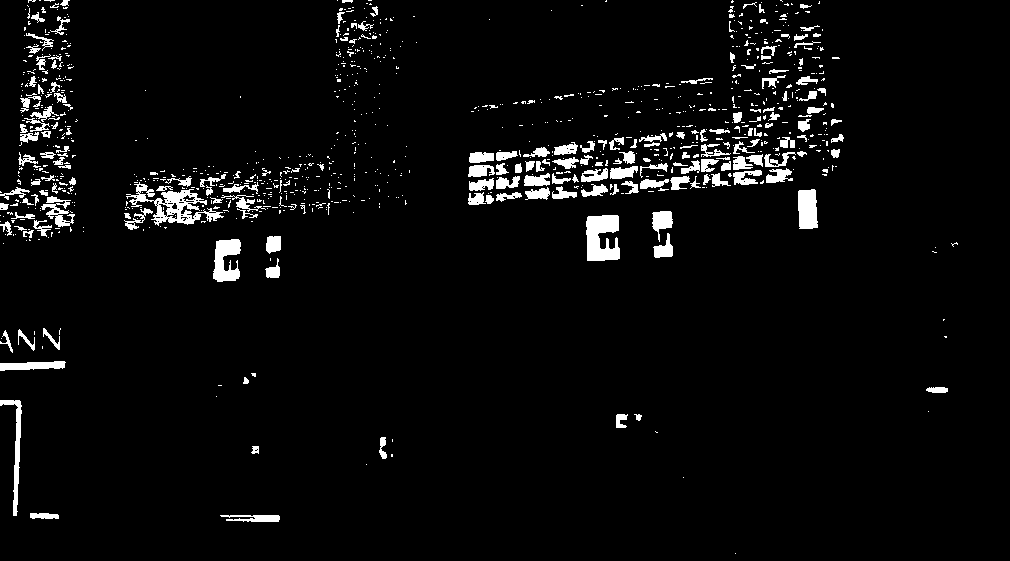
\includegraphics[width=.8\linewidth]{figures/img4_thresh_red.png}
  \caption{Czerwony}
  \label{fig:sfig1}
\end{subfigure}
\begin{subfigure}{.3\textwidth}
  \centering
  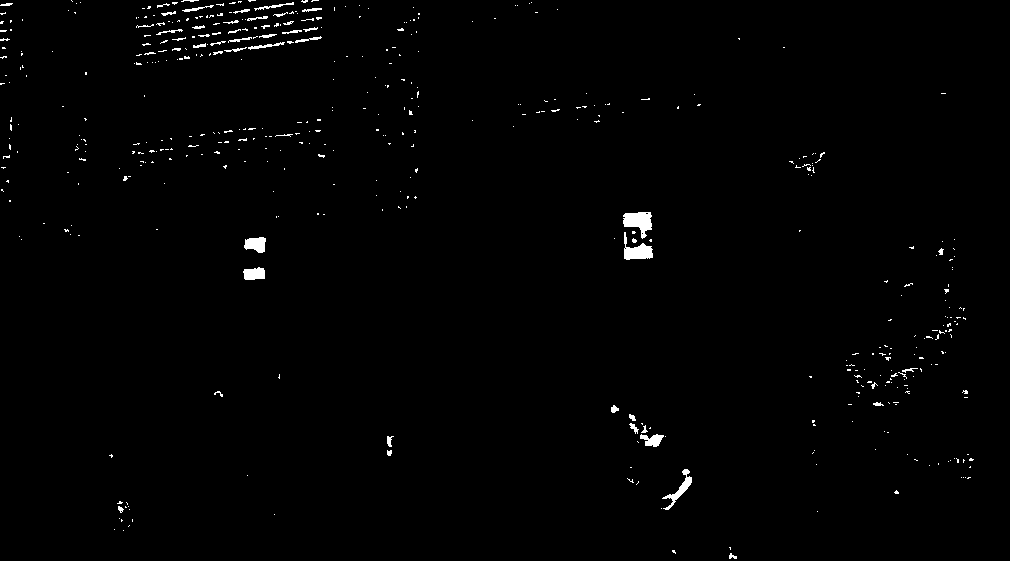
\includegraphics[width=.8\linewidth]{figures/img4_thresh_yellow.png}
  \caption{Żółty}
  \label{fig:sfig2}
\end{subfigure}
\begin{subfigure}{.3\textwidth}
  \centering
  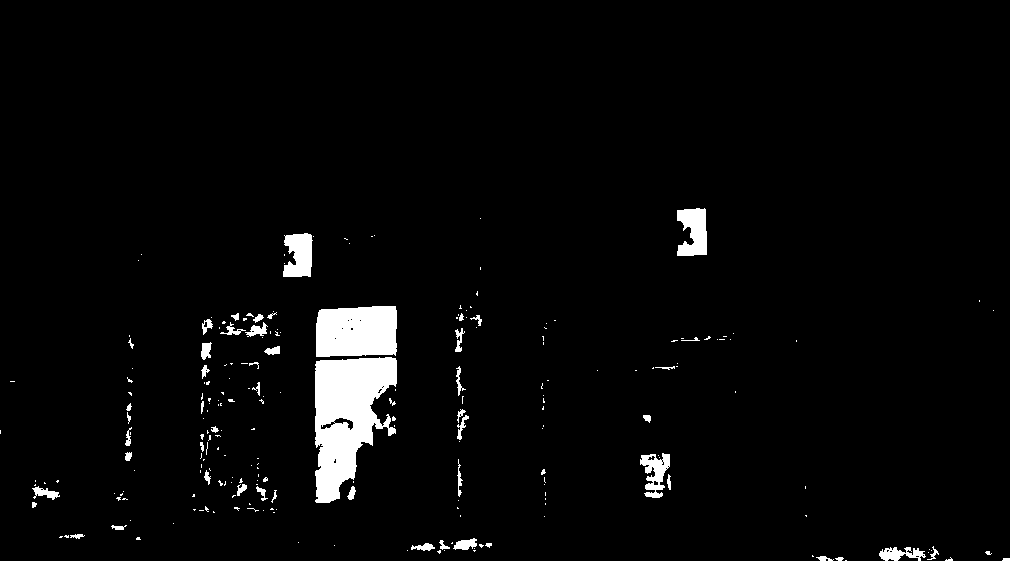
\includegraphics[width=.8\linewidth]{figures/img4_thresh_green.png}
  \caption{Zielony}
  \label{fig:sfig2}
\end{subfigure}
\caption{Binarne obrazy uzyskane po zastosowaniu progowania na obrazie \empty{d} dla poszczególnych kolorów}
\label{fig:progowanie_kolory}
\end{figure}

\subsection{Segmentacja obszarowa - rozrost obszarów}

Na tym etapie przetwarzania z jednostkowe piksele oznaczone na etapie progowania zostały pogrupowane w większe segmenty. Dokonano tego stosując implementując algorytm podążający za ogólną zasadę algorytmów typu \emph{flood fill}.

Rozpoczynając grupowanie od jednego znalezionego zaznaczonego piksela, analizowano rekursywnie sąsiadów kolejnych pikseli. Wybranym wariantem sąsiedztwa pikseli został wariant 4-pikselowy (przedstawiony na Rys. \ref{fig:pixel_4_nb}).

\begin{figure}
    \centering
    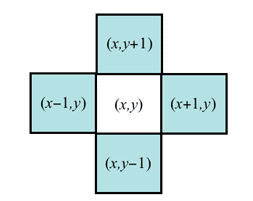
\includegraphics[width=5cm]{figures/4_pixel_neighbourhood.png}
    \caption{Wybrany wariant określający sąsiedztwo piksela}
    \label{fig:pixel_4_nb}
\end{figure}
